\documentclass[12pt]{report}

\usepackage{commands}

\begin{document}

\large

\begin{center}
 Math 585 Homework 2\\
 Due February 12\\
 By Marvyn Bailly\\
\end{center}

\normalsize

\hrule

%---------------%
%---Problem 1---%
%---------------%

%--status--$

\begin{problem}
   T1. Approximate $\pp{u}{x}|_{P_1}$ in terms of $u_0 = u(P_0), u_1 = u(P_1), u_2= u(P_2)$ (see figure, where the curve represents a quarter arc of unit circle). Estimate the error.
\end{problem}

\begin{solution}

    \noindent
    We wish to approximate $\pp{u}{x}|_{P_1}$ in terms of the given data. We pick our abscissa to be $x_0 = 0, x_1 = 1/2,$ and $x_2 = \sqrt{3}/2.$ We have the equation
    \[ 
        \pp{u}{x}|_{P_1} \approx [x_0, x_1]u + (x_0 - x_1)[x_0,x_1,x_2]u.
    \]  
    Using a divided difference table we get that $[x_0, x_1]u = 2(u_1 - u_0)$ and $[x_0,x_1,x_2]u = \frac{2}{\sqrt{3}}\paren{\frac{2}{\sqrt{3}-1}\paren{u_2 - u_1}-2(u_1 - u_0)}$. Thus we get
    \begin{align*}
        \pp{u}{x}|_{P_1} &\approx 2(u_1 - u_0) + \frac{1}{2}\cdot\frac{2}{\sqrt{3}}\paren{\frac{2}{\sqrt{3}-1}\paren{u_2 - u_1}-2(u_1 - u_0)}\\
        &= \frac{3 + \sqrt{3}}{3}u_2 -(\sqrt{3}-1)u_1 - \frac{6-2\sqrt{3}}{3}u_0.
    \end{align*} 
    Next we wish to estimate the error. We know that the error is given by
    \begin{align*}
        \text{error} &= \frac{f'''(\xi;x_1)}{6}(x_1 - x_0)(x_1 - x_2) = \frac{f'''(\xi;1/2)}{24}(1 - \sqrt{3}).
    \end{align*}
    Thus we can estimate the maximum error to be
    \[ 
        |\text{error}|\leq \max_{x_0 \leq \xi \leq x_2} \frac{\sqrt{3}-1}{24}\left|f'''(\xi;1/2)\right|.
    \]

\end{solution}

%----------------------------------------------------------------------------------------------------%
%\vskip 20pt
\newpage

%---------------%
%---Problem 2---%
%---------------%

%--status--$

\begin{problem}
    T2. Find a two-point Gauss quadrature to approximate 
    \[ 
        \int_0^1 \frac{e^x}{\sqrt{x}}\dx{x}. 
    \]
\end{problem}

\begin{solution}
    
    \noindent
    We wish to find a two-point Gauss quadrature to approximate
    \[ 
        \int_0^1 e^x \frac{1}{\sqrt{x}}\dx{x},       
        \]
        were $\frac{1}{\sqrt{x}}$ is our weight function. 
        We have that the quadrature rule is of the form
        \[ 
            \int_a^b f(x)w(x)dx = \sum_{i=0}^{n}a_if(x_i) + E_n(f).
        \]
        First we need to find a basis that is orthonormal to the weight function. Observe that by beginning with the basis $\hat{\pi}_0,\hat{\pi}_1,\hat{\pi}_2=1,x,x^2$ and apply the Gram-Schmidt algorithm yields
    \begin{align*}
        \pi_0 &= \hat{\pi}_0 = 1,\\
        \\
        \pi_1 &= \hat{\pi}_1 - \frac{\abrac{\pi_0,\hat{\pi}_1}}{\abrac{\pi_0,\pi_0}}\\
        &=x - \frac{\abrac{1,x}}{\abrac{1,1}}\\
        &= x - \frac{\int_0^1 x \cdot x^{-1/2}\dx{x}}{\int_0^1x^{-1/2}\dx{x}}\\
        &= x - \frac{2/3}{2}\\
        &= x - \frac{1}{3},\\
        \\
        \pi_2 &= \hat{\pi_2} - \frac{\abrac{\pi_1,\hat{\pi}_2}}{\abrac{\pi_1,\pi_1}}\pi_1 - \frac{\abrac{\pi_0,\hat{\pi}_2}}{\abrac{\pi_0,\pi_0}}\\
        &= x^2 - \frac{\int_0^1 (x - 1/3)(x^2)(x^{-1/2})\dx{x}}{\int_0^1(x - 1/3)^2(x^{-1/2})\dx{x}}(x - 1/3) - \frac{\int_0^1 (x^2)(x^{-1/2})\dx{x}}{\int_0^1(x - 1/3)^2(x^{-1/2})\dx{x}}\\
        &=x^2 \frac{16/105}{8/45}(x-1/3) - \frac{2/5}{2}\\
        &=x^2 - 6/7(x-1/3) - 1/5\\
        &= x^2 - \frac{6}{7}x + \frac{3}{35}.
    \end{align*}
    Picking our abscissa to be the roots of $\pi_2$ give
    \[ 
        \pi_2 = 0 \implies  x^2 - \frac{6}{7}x + \frac{3}{35} = 0 \implies x_{0,1} = \frac{15\mp 2\sqrt{30}}{35}.
    \]
    Next we wish to solve for $a_i$ which is of the form
    \[ 
        a_i = \int_0^1 l_i(x)w(x)\dx{x},
    \]
    where
    \[ 
        l_i = \prod_{j=0, j\neq i}^{n} \frac{x - x_j}{x_i - x_j}.
    \]
    Thus we have that
    \begin{align*}
        l_0 &= \frac{x - x_1}{x_0 - x_1} = \frac{x - (\frac{15 + 2\sqrt{30}}{35})}{-\frac{4\sqrt{30}}{35}} = - \frac{7\sqrt{30}}{24}\paren{x - \frac{15 + 2\sqrt{30}}{35}},\\
        l_1 &= \frac{x - x_0}{x_1 - x_0} = \frac{x - (\frac{15 - 2\sqrt{30}}{35})}{\frac{4\sqrt{30}}{35}} = \frac{7\sqrt{30}}{24}\paren{x - \frac{15 + 2\sqrt{30}}{35}}.
    \end{align*}
    Which gives
    \begin{align*}
        a_0 &= - \frac{7\sqrt{30}}{24} \int_0^1 x^{-1/2} - \frac{15 + 2\sqrt{30}}{35}x^{-1/2}\dx{x} \\
        &= - \frac{7\sqrt{30}}{24} \left[ \frac{2}{3}x^{3/2} - \frac{30 + 4\sqrt{30}}{35}x^{1/2} \right]_0^1\\
        &= - \frac{7\sqrt{30}}{24}\paren{\frac{20 + 12\sqrt{30}}{105}}\\
        &= 1 + \frac{\sqrt{30}}{18},\\
        \\
        a_1 &= \frac{7\sqrt{30}}{24} \int_0^1 x^{-1/2} - \frac{15 - 2\sqrt{30}}{35}x^{-1/2}\dx{x} \\
        &= 1 - \frac{\sqrt{30}}{18}.
    \end{align*}
    Therefore we have found the two-point Gauss quadrature approximation to be 
    \begin{align*}
        \int_a^b f(x)w(x)dx &\approx \sum_{i=0}^{n}a_if(x_i)\\
        &= a_0 f(x_0) + a_1 f(x_1)\\
        &=  \paren{1 + \frac{\sqrt{30}}{18}}e^{\frac{15 - 2\sqrt{30}}{35}} + \paren{1 - \frac{\sqrt{30}}{18}}e^{\frac{15 + 2\sqrt{30}}{35}}\\
        &\approx 2.9245.
    \end{align*} 

\end{solution}

%----------------------------------------------------------------------------------------------------%
%\vskip 20pt
\newpage

%---------------%
%---Problem 3---%
%---------------%

%--status--$

\begin{problem}
    T3. Suppose that the interval $[a, b]$ is divided into equal subintervals of length $h$ each such that $n = (b-a)/h$ is even. Denote by $R_1$ the result of applying the composite trapezoidal method with step size $2h$ and by $R_2$ the result of applying the same method with step size $h$. Show that one application of Richardson extrapolation, reading 
    \[ 
        S = \frac{4R_2 - R_1}{3}
    \]
    yields the composite Simpson method.

\end{problem}

\begin{solution}

    \noindent
    Consider the interval $[a,b]$ that is divided into equal subintervals of length $h$ each such that $n = (b-a)/h$ is even. Consider the composite trapezoidal method with a step size of $2h$ which is of the form
    \[ 
        R_1 = h\paren{f(a) + 2f(a + 2h) + \cdots + 2f(b - 2h) + f(b)},
    \]
    and with a step size of $h$ which is of the form
    \[ 
        R_2 = \frac{h}{2}\paren{f(a) + 2f(a + h) + 2f(a + 2h) + \cdots + 2f(b - 2h) + 2f(b - h) + f(b)}.
    \]
    Now notice that one application of Richardson extrapolation yields
    \begin{align*}
        S &= \frac{4R_2 - R_1}{3}\\
        &= \frac{\paren{2h(f(a) + \cdots + f(b))} - \paren{h}(f(a) + \cdots + f(b))}{3}\\
        &= \frac{h}{3}\big[ (2f(a) - f(a)) + 4f(a+h) + (4f(a + 2h) - 2f(a+2h))\\
        &+ \cdots + (4f(b - 2h) - 2f(b-2h)) + 4f(b-h) + (2f(b) - f(b))\big]\\
        &= \frac{h}{3} \paren{ f(a) + 4f(a + h) + 2f(a +2h) + \cdots + 2f(b-2h) + 4f(b-h) + f(b)},
    \end{align*}
    which is the form of the composite Simpson method. Note that on each $2h$ step, we have a perfect alignment between $R_2$ and $R_1$ since we required that there are an even amount of subintervals. Thus we can always subtract terms on the $2h$ step to get the alternating $4$ and $2$ pattern seen in Simpson method.  
\end{solution}

%----------------------------------------------------------------------------------------------------%
%\vskip 20pt
\newpage

%---------------%
%---Problem 4---%
%---------------%

%--status--$
\begin{figure}
    \center
    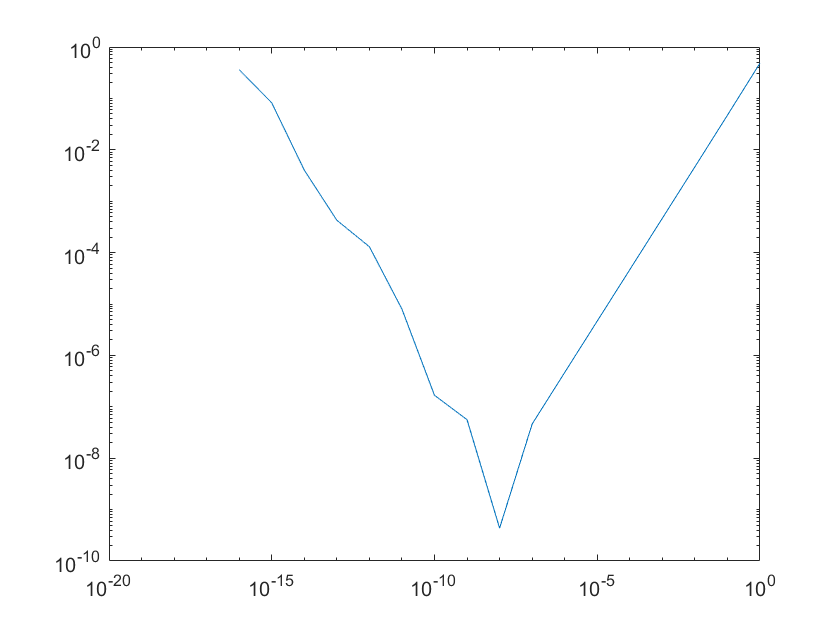
\includegraphics[width=.8\textwidth]{plots/c1a.png}
    \caption{The absolute error vs. $h$ on a loglog plot.}
\end{figure}
\begin{problem}
    C1. One can approximate the derivative of a function $f(x)$ by
    \[ 
        f'(x) \approx \frac{f(x + h) - f(x)}{h}.
    \]
    In class, we derived that
    \[ 
        \left| f'(x) - \frac{f(x + h) - f(x)}{h}\right| = \O(h).
    \]
    Let $f(x) = \sin(x)$. 
    \begin{enumerate}
        \item [(a)] Approximate $f'(x)$ at $x_0 = 1.2$ Take \verb+h = 10.^i; u = 0:-1:-16+ and plot the absolute error $\left| f'(x_0) - \frac{f(x_0 + h) - f(x_0)}{h} \right|$ vs. $h$ using \verb+loglog+. Does the plot behave as you expect? Explain.
        \item [(b)] By the trig identity $\sin(\alpha) - \sin(\beta) = 2\cos\paren{\frac{\alpha + \beta}{2}}\sin\paren{\frac{\alpha - \beta}{2}}$, one has
        \[ 
            \frac{f(x_0 + h) - f(x_0)}{h} = \frac{2\cos\paren{x_0 + \frac{h}{2}}\sin\paren{\frac{h}{2}}}{h}.
        \]
        Use this formula to approximate $f'(x)$ at $x_0 = 1.2$. Make the same plot as in (a). Does the plot behave as you expect? Explain.
    \end{enumerate}
\end{problem}
\begin{figure}[H]
    \center
    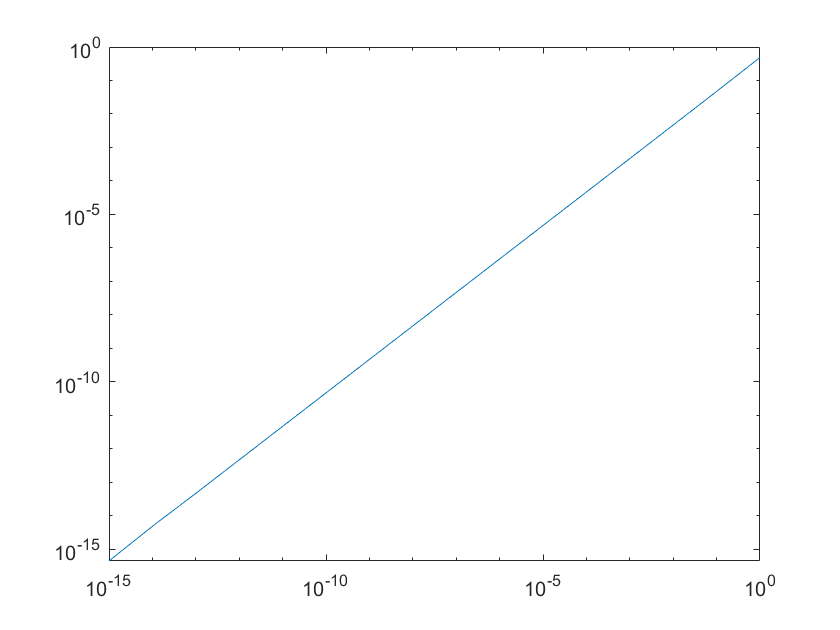
\includegraphics[width=.8\textwidth]{plots/c1b.png}
    \caption{The absolute error vs. $h$ on a loglog plot using the updated method.}
\end{figure}
\begin{solution}



    \noindent
    Consider the function $f(x) = \sin(x)$. We wish to use 
    \[ 
        f'(x) \approx \frac{f(x + h) - f(x)}{h},
    \]
    to approximate $f'(x)$ at $x_0 = 1.2$. 
    
    \begin{enumerate}
        \item 
        Using the MATLAB code I wrote in Listing 1. part A, I produced the Figure 1 which shows the absolute error $\left| f'(x_0) - \frac{f(x_0 + h) - f(x_0)}{h} \right|$ vs. $h$ on a \verb+loglog+ plot. In Figure 1. we see that at some point, the round-off error takes over the truncation error, causing the error to increase while $h$ decreases. Assuming that
        \begin{align*}
            \hat{\sin}(x_0 + h) =& \sin(x_0 + h) \eps_1,\\
            \hat{\sin}(x_0) = &\sin(x_0) \eps_2,\\
        \end{align*}
        where $|\eps_{1,2}| \leq \eps_{\text{mach}}$. Thus we have
        \begin{align*}
            f'(x_0) &= \frac{ \hat{\sin}(x_0 + h) - \hat{\sin}(x_0)}{h} + \frac{\eps_2 - \eps_1}{h} + \frac{\sin(\xi(x_0))}{2}h,\\
            \implies &\left| f'(x_0) - \frac{ \hat{\sin}(x_0 + h) - \hat{\sin}(x_0)}{h}\right| \leq \frac{2\eps_{\text{mach}}}{h} + \frac{h}{2}.
        \end{align*}
        Then the point where the round-off error takes over is when the truncation error is approximately equal to the rounding error,
        \[ 
            \frac{2\eps_{\text{mach}}}{h} = \frac{h}{2} \implies h = 2\sqrt{\eps_{\text{mach}}} \approx 10^{-8}.
        \]
        This is what we see in Figure 1.

        \item 
        To fix the cancellation error in the numerator, we use the trig identity $\sin(\alpha) - \sin(\beta) = 2\cos\paren{\frac{\alpha + \beta}{2}}\sin\paren{\frac{\alpha - \beta}{2}}$, which gives
        \[ 
            \frac{f(x_0 + h) - f(x_0)}{h} = \frac{2\cos\paren{x_0 + \frac{h}{2}}\sin\paren{\frac{h}{2}}}{h}.
        \]
        I applied this method in Listings 1. Part B to produce the Figure 2. where we see that the error decreases with $h$ but no longer blows up. 
    \end{enumerate}



    \lstinputlisting[language=Matlab,caption=MATLAB code to generate graphs]{c1.m}
\end{solution}

%----------------------------------------------------------------------------------------------------%
%\vskip 20pt
\newpage

%---------------%
%---Problem 5---%
%---------------%

%--status--$

\begin{figure}
    \center
    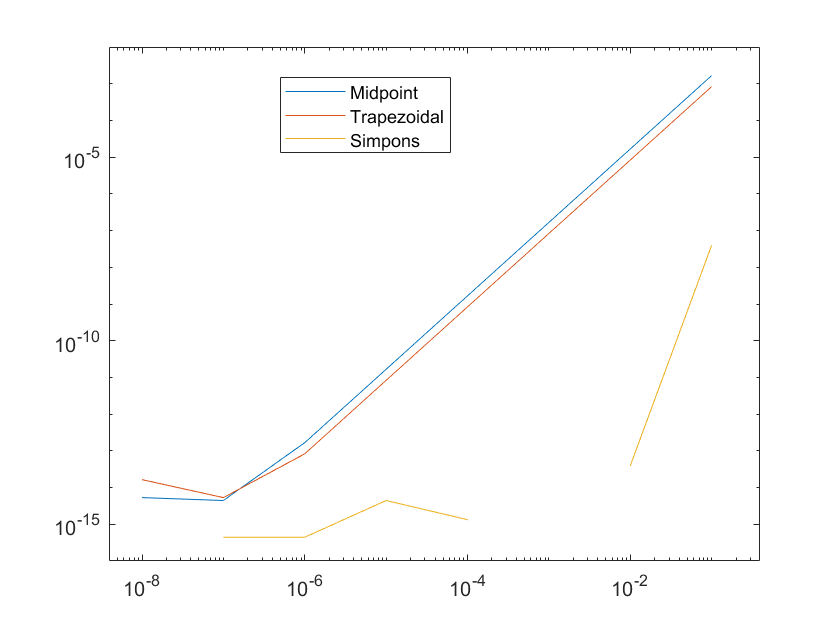
\includegraphics[width=.8\textwidth]{plots/c2.png}
    \caption{Plot of absolute error vs $h$ on a loglog plot using compute midpoint, trapezoidal, and Simpon's rule.}
\end{figure}

\begin{problem}
    C2. Suppose we know
    \[ 
        \int_0^1 \frac{4}{1+x^2}\dx{x} = \pi.
    \]
    Use the composite midpoint rule, composite trapezoidal rule, and composite Simpson's rule to approximate the above integral. Plot the error of each method w.r.t. \verb+h = 10.^i; i = -1:-1:-8+.
\end{problem}

\begin{solution}

    \noindent
    We wish to approximate
    \[ 
        \int_0^1 \frac{4}{1+x^2}\dx{x} = \pi,
    \]
    using the composite midpoint rule, composite trapezoidal rule, and composite Simpson's rule to approximate the above integral. Using the MATLAB code I created in Listings 2. I produced Figure 3. which shows the absolute error  $\left| f'(x_0) - \frac{f(x_0 + h) - f(x_0)}{h} \right|$ vs. $h$ on a \verb+loglog+ plot. Figure 3. shows that the midpoint and trapezoidal rule produce similar approximations to the integral that have absolute error which reduce with $h$ until they appear to hit machine precision and truncation error takes over at the very end. On the other hand, the Simpson's method has significantly less absolute error and even exactly approximates the integral up to machine precision at one point.     


    \center
    \lstinputlisting[language=MATLAB, caption = code to generate graphs,caption=MATLAB code to generate graphs]{c2.m}
\end{solution}

%----------------------------------------------------------------------------------------------------%
%\vskip 20pt
\newpage

\end{document}